\documentclass[12pt]{article}
\usepackage{amsmath,amsxtra,amssymb,latexsym, amscd,amsthm}
\usepackage{indentfirst}
\usepackage[mathscr]{eucal}
\usepackage[utf8]{vietnam}
\usepackage{graphicx,color}
\usepackage{fancyhdr}
\usepackage{algorithm}
\usepackage[noend]{algpseudocode}
\usepackage{animate}
\usepackage{spverbatim}
\usepackage{subcaption}
\usepackage{hyperref}
\hypersetup{
    colorlinks=true,
    linkcolor=blue,
    filecolor=magenta,      
    urlcolor=cyan,
}
\pagestyle{fancyplain}
\pagestyle{fancy}
\textheight 22truecm %%16.2truecm 
\textwidth 14truecm 
\parskip 3pt
\headsep=12pt
\renewcommand{\headwidth}{\textwidth}
\renewcommand{\sectionmark}[1]{\markright{\it \thesection. #1}}
\lhead[\fancyplain{}{\thepage}]{\fancyplain{}{\rightmark}}
\rhead[\fancyplain{}{\leftmark}]{\fancyplain{}{\thepage}}
\cfoot{}
\sloppy
\makeatletter\@addtoreset{section}{part}\makeatother %.......
\begin{document}
  \input biasach.tex
  \newpage
  \vspace*{2cm}
  \section*{LỜI MỞ ĐẦU} 
    Nội dung chủ yếu tập trung vào phần giải thuật và cách cài đặt trên ứng 
    dụng Maple, để giải quyết bài toán tìm tập bao lồi  
    trên mặt phẳng với thuật toán chuỗi đơn điệu - Monotone chain  
    
    Phiên bản sử dụng là Maple 17.
    
    Xin chân thành cám ơn sự giúp đỡ chỉ bảo tận tình của phó giáo sư Nguyễn Hữu 
    Điển. 

    Rất mong được sự góp ý của thầy cô và bạn bè. 
    
    Mọi đóng góp xin gửi về địa chỉ email : ntanhtm@gmail.com
    
    Sinh viên trình bày: \textbf{Nguyễn Tú Anh }

    Lớp : \textbf{Toán Tin ứng dụng TM29 }
  \newpage
  \tableofcontents
  \newpage
  \part {Bài toán bao lồi và thuật toán Monotone chain}
    \section{Giới thiệu bao lồi 2D}
      \subsection{Định nghĩa} 
        Trong hình học tính toán (computational geometry), 
        bao lồi (convex hull) của một tập điểm là tập lồi nhỏ nhất (theo diện tích, thể tích, ...) mà tất cả các điểm đều nằm trong tập đó.
        \begin{figure}[!ht]
          \centering
          \begin{subfigure}[b]{0.35\linewidth}
            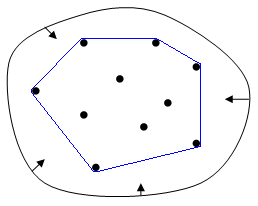
\includegraphics[width=\linewidth]{Image/ConvexHull}
            \caption{Bao lồi 2D.}
            \label{fig:ch2d}
          \end{subfigure}
          \begin{subfigure}[b]{0.35\linewidth}
            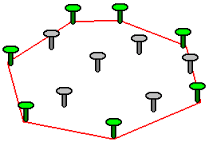
\includegraphics[width=\linewidth]{Image/ch_nail}
            \caption{Tập đinh.}
            \label{fig:chnail}
          \end{subfigure}
          \caption{}
        \end{figure}
      \subsection{Giải thích trực quan về bao lồi trên mặt phẳng}
        Sau đây là một số giải thích trực quan về bao lồi trên mặt phẳng. 
        \begin{itemize}
          \item Nếu ta coi các điểm trong một tập hợp là các cái đinh đóng trên một tấm gỗ, bao lồi của tập điểm đó có viền ngoài tạo bởi sợi dây chun mắc vào các cái đinh sau khi bị kéo căng về các phía. (Hình \ref{fig:chnail})
          \item Nếu ta coi các điểm trong một tập hợp là các con cừu trên đồng cỏ, bao lồi của tập điểm đó có viền ngoài là hàng rào có độ dài nhỏ nhất bao quanh tất cả các con cừu.
          \item Nếu ta coi các điểm trong một tập hợp là các đầu mút có thể của các hàng rào, bao lồi của tập điểm đó có viền ngoài là các hàng rào thẳng có điểm đầu và điểm cuối thuộc tập điểm đó và bao quanh diện tích lớn nhất.
        \end{itemize}
    \section{Thuật toán tìm bao lồi - Monotone chain}
      Bài toán tìm bao lồi của một tập điểm trên mặt phẳng là một trong những bài toán được nghiên cứu nhiều nhất trong hình học tính toán và có rất nhiều thuật toán để giải bài toán này. Sau đây là thuật toán tìm bao lồi trên mặc phẳng có tốc dộ nhanh và phổ biến nhất - Monotone chain.
      \subsection{Giới thiệu}
        Thuật toán Monotone chain của Andrew xây dụng tập điểm bao lồi của một tập điểm trên mặt phằng (2-dimensional points) với độ phức tập thuật toán $O(n\log n)$.
      \subsection{Nguyên lý}
        \begin{figure}[!ht]
          \centering
          \begin{subfigure}[b]{0.4\linewidth}
            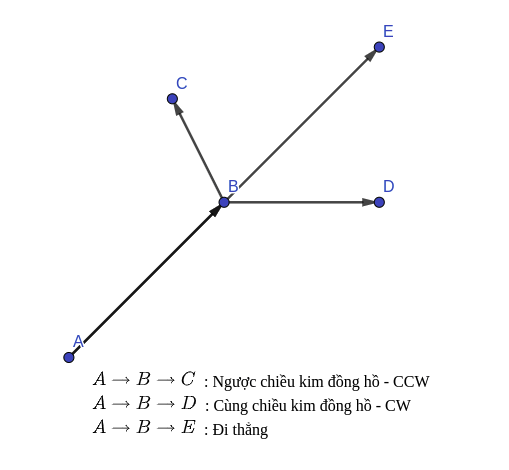
\includegraphics[width=\linewidth]{Image/cw}
            \caption{Hướng kim đồng hồ.}
            \label{fig:ccw} 
          \end{subfigure}
          \begin{subfigure}[b]{0.4\linewidth}
            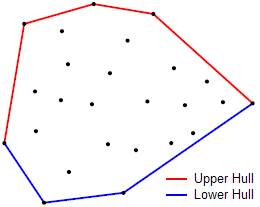
\includegraphics[width=\linewidth]{Image/upperandlower}
            \caption{Bao lồi trên và dưới}
            \label{fig:uplow} 
          \end{subfigure}
          \caption{}
        \end{figure}
        Thuật toán dựa trên việc tìm hai chuỗi đơn điệu của bao lồi: chuỗi trên và chuỗi dưới. 
        Ta thấy điểm ở xa về phía bên phải nhất (từ đây gọi là điểm phải nhất) và điểm ở xa về phía bên trái nhất 
        (từ đây gọi là điểm trái nhất) trong dữ liệu vào luôn là hai đỉnh của bao lồi. 
        Phần bao lồi theo chiều kim đồng hồ (Hình \ref{fig:ccw}) tính từ điểm trái nhất và ngược chiều kim đồng hồ tính từ điểm phải nhất gọi là chuỗi trên, 
        phần còn lại của bao lồi gọi là chuỗi dưới.
        Ta sẽ tìm chuỗi trên và chuỗi dưới độc lập với nhau.
      \newpage
      \subsection{Thuật toán}
        Các bước tiến hành thuật toán Monotone chain như sau:
        \begin{itemize}
          \item Bước đầu tiên là sắp xếp các điểm được cho theo thứ tự tăng dần theo hoành độ. Nếu hai điểm có cùng hoành độ, điểm có tung độ nhỏ hơn sẽ đứng trước. Trong thời gian $0(n \log n)$
          \item Ta xét việc xây dựng chuỗi trên với độ phức tạp $O(n)$. 
            Gọi $H$ là chuỗi bao lồi trên hiện tại đã tìm được và độ lớn của bao là $h$. Điểm đầu của chuỗi là $H_1$ và điểm cuối là $H_h$. Với mỗi điểm $P$ được xét:
            \begin{itemize}
              \item[B1.] Nếu $h < 2$ xét điểm tiếp theo.
              \item[B2.] Gọi $\overrightarrow{\rm u} = \overrightarrow{\rm H_{h-1}H_{h}}$ và $\overrightarrow{\rm v} = \overrightarrow{\rm H_hP}$. 
                Do ta đang di chuyển theo chiều kim đồng hồ nên để tìm chuỗi trên nên ta kiểm tra xem $\overrightarrow{u}x\overrightarrow{v}$ có nhỏ hơn 0 hay không.
                Nếu có ta xét điểm tiếp theo, nếu không ta loại bỏ $H_h$ quay lại bước B1.
              \item[B3.] Thêm điểm $P$ vào $H$
            \end{itemize}
          \item Việc xây dựng chuỗi bao lồi dưới tương tụ. Ta sẽ được kết quả như hình \ref{fig:uplow}
        \end{itemize}
      \newpage
      \subsection{Giả mã (Pseudo-code)}
        Gồm 2 thuật toán chính đó là "Kiểm tra đi ngược chiều kim đồng hồ " (Algorithm 1) và thuật toán tìm tập bao lồi Monotone chain (Algorithm 2). Giải thích rõ hơn sẽ được viết trong phần II.
        \begin{algorithm}2
          \caption{Check Counter-clockwise}
          \begin{algorithmic}[1]
            \Procedure{isCCW}{$p_1$, $p_2$, $p_3$}
              \State d = $\overrightarrow{p_1p_2}$ x $\overrightarrow{p_2p_3}$
              \If{ d > 0} \Return true
              \Else \text{ } \Return false 
              \EndIf
            \EndProcedure
          \end{algorithmic}
        \end{algorithm}
        \begin{algorithm}
          \caption{Convex Hull}
          \begin{algorithmic}[1]
            \Procedure{ConvexHull}{list P of points}
              \State $\textbf{Sort}$ the points of P by x-coordinate (in case of a tie, sort by y-coordinate).
              \State Initialize U and L as empty lists.
              \State Constructing upper hulls - U
              \For{i = 1..n}
                \While{sizeof(U) >= 2}{
                  \If {isCCW(U[h-1],U[h],P[i]) == true }
                    \State Delete the $h_{th}$ element of U - U[h]
                  \Else \State Break loop
                  \EndIf
                }
                \EndWhile
                \State append P[i] to U
              \EndFor
              \State Constructing lower hulls - L
              \For{i = n..1}
                \While{sizeof(L) >= 2}{
                  \If {isCCW(L[k-1],L[k],P[i]) == true}
                    \State Delete the $k_{th}$ element of L - L[k]
                  \Else \State Break loop
                  \EndIf
                }
                \EndWhile
                \State append P[i] to L
              \EndFor  
              \State Remove the first and last point of L.
              \State Concatenate L and U to obtain the convex hull of P.
              \State Points in the result will be listed in counter-clockwise order.
            \EndProcedure
          \end{algorithmic}
        \end{algorithm}
  %...
  \newpage
  \part{Biểu diễn bài toán với Maple}
    \section{Mã nguồn}
      Mã nguồn được viết và thể hiện bằng ứng dụng Maple. Gồm 2 hàm chính là: "isCCW", "ConvexHull" để tìm tập bao lồi và 3 hàm phụ giúp ta có thực nghiệm rõ ràng hơn.
      \subsection{Hàm chính}
      \subsubsection{Hàm "isCCW"}
        Hàm kiểm tra hướng đi của vector, được sử dụng trong việc tìm bao lồi trên và dưới.
        \begin{itemize}
          \item Mô tả:
          \begin{itemize}
            \item Tham số: Gồm 3 điểm - a, b, c với a[1], a[2] lần lượt là tọa độ x, y của điểm a 
            \item Trả về: boolean (true or false)
            \item Độ phức tạp thuật toán: $O(1)$
            \item Nhiệm vụ: Kiểm tra hướng đi từ điểm b đến c có đi theo hướng cùng chiều kim đồn hồ hay không ? (Đã đi từ a đến b)
          \end{itemize}
        \item Code by Maple 
        \begin{verbatim}
  isCCW := proc(a,b,c)
    #counterclockwise
    local d;
    d := a[1]*(b[2] - c[2]) + b[1]*(c[2] - a[2]) + c[1]*(a[2]-b[2]):
    if d > 0 then return true; else return false; fi:
  end proc:
        \end{verbatim}
      \end{itemize}
        \newpage
      \subsubsection{Hàm "ConvexHull"}
        Hàm tìm tập bao lồi của 1 danh sách điểm đưa vào sử dụng thuật toán Monotone chain với thời gian $O(n \log n)$
        \begin{itemize}
          \item Mô tả:
          \begin{itemize}
            \item Tham số: Danh sách điểm cần tìm bao lồi (2-D)
            \item Trả về: Danh sách điểm nằm trên bao lồi 
            \item Độ phức tạp thuật toán: $O(n\log n)$
            \item Nhiệm vụ: Tìm tập điểm nằm trên bao lồi được liệt kê theo hướng cùng chiều kim đồng hồ
          \end{itemize}
        \item Code by Maple:
        \begin{verbatim}
  ConvexHull := proc(P)
    local res,up,low,nUp,nlow,nPo,i,j,Ps:
    Ps := {op(P)}; #Chuyển về tập set để sắp xếp, loại bỏ lặp
    nUp := 0: nlow := 0: nPo := nops(Ps):
    up := vector(nPo): low:= vector(nPo):
    for i from 1 to nPo do:
      while nUp >= 2 do:
        if isCCW(up[nUp-1],up[nUp],Ps[i]) then nUp := nUp - 1;
        else break; fi;
      od:
      nUp := nUp + 1; up[nUp] := Ps[i]:
    od:
    for i from nPo by -1 to 1 do:
      while nlow >= 2 do:
        if isCCW(low[nlow-1],low[nlow],Ps[i]) then nlow := nlow - 1:
        else break: fi:
      od:
      nlow := nlow + 1: low[nlow]:= Ps[i]:
    od:
    res := vector(nUp + nlow - 2):
    for i from 1 to nUp do: res[i] := up[i]: od:
    for j from 2 to nlow-1 do: res[j - 1 + nUp]:= low[j]: od:
    return convert(res,list):
  end proc:
        \end{verbatim}
      \end{itemize}
        \newpage
    \subsection{Hàm phụ}
      \subsubsection{Hàm 'RandPoints'}
        Hàm tạo tập điểm ngẫu nhiên cho thực nhiệm. Khả dụng sinh $10^6$ điểm nhưng với độ phức tạp $O(n \log n)$ của thuật toán chỉ nên tạo $10^5$ điểm.
        \begin{itemize}
          \item Mô tả: 
          \begin{itemize}
            \item Tham số: Gồm 3 tham số
              \begin{itemize}
                \item n: Số lượng điểm
                \item $range_x$: Khoảng giới hạn của tọa độ x - $(x_{min}..x_{max})$ 
                \item $range_y$: Khoảng giới hạn của tọa độ y - $(y_{min}..y_{max})$ 
              \end{itemize}
            \item Kiểu trả về: Danh sách n điểm thỏa mãn điều kiện 
            \item Độ phức tạp thuật toán: $O(n)$
            \item Nhiệm vụ: Sinh n điểm ngẫu nhiên
          \end{itemize}
        \item Code by Maple
          \begin{verbatim}
  RandPoints := proc(n,range_x,range_y)
    local P,roll, i, x, y:
    P:= vector(n): d:= 1:
    roll_x := rand(range_x);
    roll_y := rand(range_y);
    for i from 1 to n do:
      x:= roll_x(): y:= roll_y():
      P[d] := [x,y]: d:= d+1:
    end do:
    return convert(P,list):
  end proc:
          \end{verbatim}
        \end{itemize}
        \newpage
      \subsubsection{Hàm 'myPlot'}
        Hàm làm nhiệm vụ đơn giản nhưng phải có vì cần sử dụng trong hàm "animate" của Maple giúp vẽ hình ảnh động.
        \begin{itemize}
          \item Mô tả:
          \begin{itemize}
            \item Tham số: 1 số nguyên - i và danh sách plots - listPlots
            \item Kiểu trả về: plot 
            \item Độ phức tạp thuật toán: $O(1)$
            \item Nhiệm vụ: Lấy plot thứ i của danh sách listPlots
          \end{itemize}
          \item Code by Maple
            \begin{verbatim}
  myPlot := (p,listPlots) ->  listPlots[trunc(p)];
            \end{verbatim}
        \end{itemize}
      \subsubsection{Hàm 'AniConvexHull'}
        Hàm tạo ảnh động thể hiện các bước thực hiện của thuật toán. Vì đâu là ảnh động biểu diễn trực quan nên chỉ khả dụng với tập điểm với số lượng điểm \textbf{nhỏ hơn 50} !
        \begin{itemize}
          \item Mô tả:
          \begin{itemize}
            \item Tham số: Danh sách điểm - P, Tùy chọn Axes và Scaling 
            \item Kiểu trả về: 3 plot(2 plot là animate) 
            \item Nhiệm vụ: Tạo ảnh động thể hiện các bước đi của thuật toán
          \end{itemize}
          \item Code by Maple
            \begin{spverbatim}
  AniConvexHull := proc(P,Axes,Scaling)
    local res, up, low, nUp, nlow, nPo, nPl, i, j, Ps, p, l, aniUp, aniLow:
    Ps := {op(P)}:
    nPo := nops(Ps):
    up := vector(nPo): low:= vector(nPo):
    Plots := vector(5*nPo):
    nPl := 0:
    p := pointplot([Ps[1],Ps[nPo]], color = red,symbol = solidcircle, symbolsize = 30, axes = Axes, scaling = Scaling):
    bg := display(pointplot(P,symbol = solidcircle, symbolsize = 15, axes = Axes, scaling = Scaling),p):
    Plots[1] := p: nPl := 1:
    #-------Up---------#
    up[1] := Ps[1]: nUp:= 1:
    for i from 2 to nPo do:
      p := display(p, line(up[nUp], Ps[i], color = red, thickness= 3));
      nPl := nPl + 1: Plots[nPl] := p:
      while nUp >= 2 do:
        if isCCW(up[nUp-1],up[nUp],Ps[i]) then
          l := line(up[nUp],Ps[i],color = gray, thickness= 3);
          p := display(p,l): nPl := nPl + 1: Plots[nPl] := p:
          l := line(up[nUp-1],up[nUp],color = gray, thickness= 3);
          p := display(p,l): nPl := nPl + 1: Plots[nPl] := p:
          l := line(up[nUp-1],Ps[i],color = red,thickness= 3);
          p := display(p,l): nPl := nPl + 1: Plots[nPl] := p:
          nUp := nUp - 1:
        else break: fi:
      od:
      nUp := nUp + 1: up[nUp] := Ps[i]:
    od:
    aniUp := animate(myPlot,[t,Plots],t=1..nPl,background=bg, frames = nPl, title="Convex Hull - Up");
    #-------low---------#
    p := pointplot([Ps[1],Ps[nPo]],color = red,symbol = solidcircle, symbolsize = 30, axes = Axes, scaling = Scaling):
    Plots[1] := p: nPl := 1:
    low[1] := Ps[nPo]: nlow := 1:
    for i from nPo - 1 by -1 to 1 do:
      p := display(p, line(low[nlow], Ps[i], color = red, thickness= 3));
      nPl := nPl + 1: Plots[nPl] := p:
      while nlow >= 2 do:
        if isCCW(low[nlow-1],low[nlow],Ps[i]) then 
          l := line(low[nlow],Ps[i],color = gray, thickness= 3);
          p := display(p,l): nPl := nPl + 1: Plots[nPl] := p:
          l := line(low[nlow-1],low[nlow],color = gray, thickness= 3);
          p := display(p,l): nPl := nPl + 1: Plots[nPl] := p:
          l := line(low[nlow-1],Ps[i],color = red,thickness= 3);
          p := display(p,l): nPl := nPl + 1: Plots[nPl] := p:
          nlow := nlow - 1:
        else break: fi:
      od:
      nlow := nlow + 1: low[nlow]:= Ps[i]:
    od:
    aniLow := animate(myPlot,[t,Plots],t=1..nPl,background=bg, frames = nPl,title="Convex Hull - low");
    res := vector(nUp + nlow - 2):
    for i from 1 to nUp do: res[i] := up[i]: od:
    for j from 2 to nlow-1 do: res[j - 1 + nUp]:= low[j]: od:
    poly := polygon(convert(res,list),linestyle = solid, color = "white",thickness= 3);
    return [aniUp,aniLow,display(poly,bg)]:
  end:
            \end{spverbatim}
            \newpage
        \end{itemize}
    \section{Thực nghiệm} 
        \begin{figure}
          \centering
          \begin{subfigure}[h]{0.4\linewidth}
            
\includegraphics[width=\linewidth]{Image/randPoint}
            \caption{Tập điểm}
            \label{fig: points}
          \end{subfigure}
          \begin{subfigure}[h]{0.4\linewidth}
            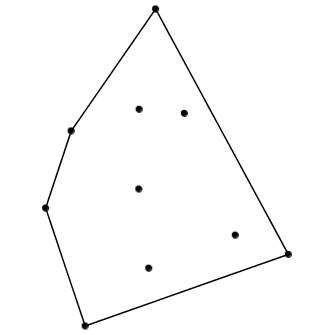
\includegraphics[width=\linewidth]{Image/polych}
            \caption{Bao lồi}
            \label{fig: polych}
          \end{subfigure}
          \caption{Thực nghiệm}
        \end{figure}
        \subsection*{Sinh ngẫu nhiên danh sách điểm}
          \subsubsection*{Lệnh}
            \begin{spverbatim}
    >Points := RandPoints(10,-800 .. 900, -1000 .. 1200): [1]
    >display(point(Points,symbol = solidcircle, symbolsize = 15),axes = Axes, scaling = Scaling)); [2]
            \end{spverbatim}
          \subsubsection*{Giải thích}
            \begin{itemize}
              \item [1]: Sinh ngẫu nhiên 10 điểm với tọa độ x nằm trong khoảng -800 đến 900 và tọa độ y trong khoảng -1000 đến 1200 sau đó gán và biến Points.
              \item [2]: Vẽ plot các điểm vừa tạo.
            \end{itemize}
          \subsubsection*{Kết quả} 
            Kết quả ta sẽ có 1 plot thể hiện 10 điểm được sinh ngẫu nhiên như hình \ref{fig: points}
            \newpage
        \subsection*{Tìm bao lồi}
            \subsubsection*{Lệnh}
              \begin{spverbatim}
  >p:= ConvexHull(Points): [1]
  >poly := polygon(p,linestyle = solid, color = "White" ): [2]
  >display(poly,point(Points,symbol = solidcircle, symbolsize = 15),axes = Axes, scaling = Scaling)); [3]
              \end{spverbatim}
            \subsubsection*{Giải thích}
              \begin{itemize}
                \item [1]: Thực hiện thuật toán trả về tập bao lồi của danh sách điểm Points vừa tạo ở trên gắn vào biến p
                \item [2]: Do danh sách điểm được liệt kê theo chiều kim đồng hồ, nên ta dễ dàng vẽ được 1 đa giác từ tập điểm đó dùng hàm "polygon" trong Maple.
                \item [3]: Dùng "display" để thể hiện đa giác vừa tìm được và tập điểm ban đầu.
              \end{itemize}
            \subsubsection*{Kết quả}
              Kết quả giống ta sẽ có 1 đa giác lồi bao 10 điểm đã tạo ở trên như hình \ref{fig: polych}
              \newpage
        \subsection*{Vẽ ảnh động các bước đi của thuật toán}
          \subsubsection*{Lệnh}
            \begin{spverbatim}
    >listPlots := AniConvexHull(Points,Axes,Scaling):  [1]
    >listPlots[1]; listPlots[2]; [2]
            \end{spverbatim}
          \subsubsection*{Giải thích}
            \begin{itemize}
              \item [1]: Sử dụng hàm "AniConvexHull" để vẽ ảnh động cho bước đi của thuật toán với tập điểm Points và 2 tùy chọn của plot
              \item [2]: Thể hiện 2 plot bao lồi trên và dưới.
            \end{itemize}
        \subsubsection*{Kết quả}
          \begin{frame}{}
            \centering
            \animategraphics[loop,autoplay,width=7cm]{1}{GIF/Up-}{0}{27}
            \animategraphics[loop,autoplay,width=7cm]{1}{GIF/Low-}{0}{30}
          \end{frame}
          \\
          \begin{center}
            Chú ý: Ảnh động khả dụng khi đọc bởi "Adobe Reader" !
          \end{center}
        \newpage
    \section{Giao diện trong ConvexHullSuper.mw}
      \subsection{Mã nguồn}  
        Mã nguồn được viết trong phần "Startup Code" (Ctrl + Shift + E)
        của file.
        \begin{figure}[h!]
          \centering
          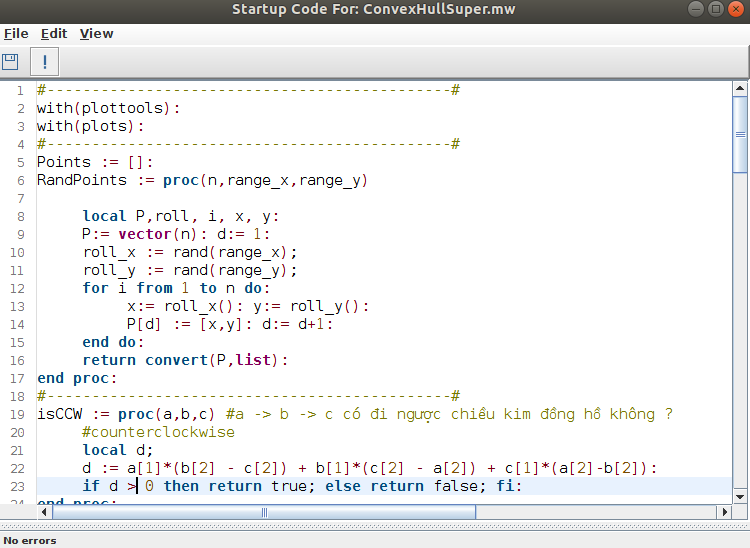
\includegraphics[scale=0.5]{Image/codeMaple}
        \end{figure}
        \newpage
      \subsection{Giao diện chính}
        Giao diện được viết bằng DocumentTools[Components] của Maple
        \subsubsection{Tạo danh sách điểm}
          Sau khi điền các tùy chọn thì kích vào nút "Update Plot" để thực hiện khởi tạo tập điểm như mong muốn.
          \begin{figure}[h]
            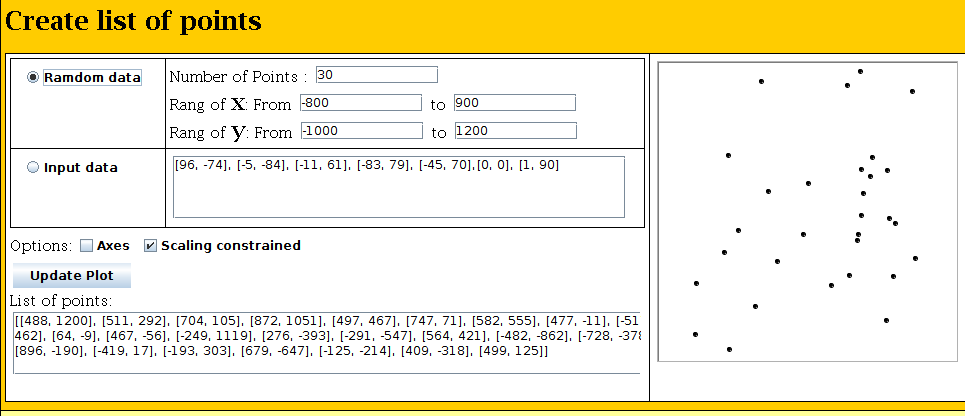
\includegraphics[scale=0.4]{Image/create}
          \end{figure}
        \subsubsection{Tìm bao lồi và vẽ đa giác}
          Kích vào nút "Start Convex Hull" để bắt đầu tìm bao lồi từ tập điểm khởi tạo ở trên.
          \begin{figure}[h]
            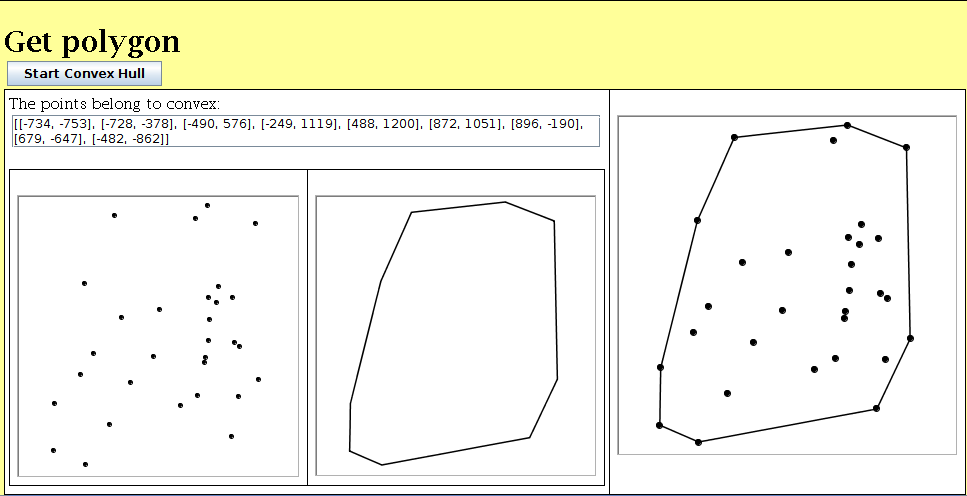
\includegraphics[scale=0.4]{Image/poly}
          \end{figure}
        \subsubsection{Vẽ ảnh động thể hiện các bước của thuật toán}
          Kích vào nút "Performing" để vẽ ảnh động.
          \begin{figure}[h]
            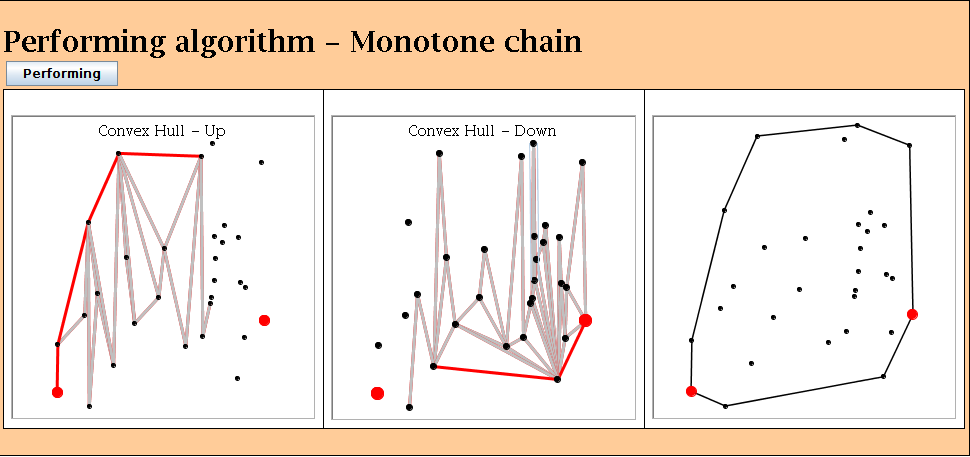
\includegraphics[scale=0.4]{Image/ani}
          \end{figure}
    \section{Kết luận}
    \begin{itemize}
      \item Thuật toán chuỗi đơn điệu (Monotone chain) vừa dễ cài đặt, vừa là thuật toán nhanh nhất trong các thuật toán tìm bao lồi trên mặt phẳng (Quan điểm cá nhân). 
      \item Maple là phần mềm toán học kết hợp công cụ toán học mạnh nhất thế giới với giao diện giúp dễ dàng phân tích, khám phá, trực quan hóa và giải quyết các vấn đề toán học.
      Dễ dàng thể hiện các bước thuật toán, và rất dễ lập trình.
      Mọi thứ trở lên trực quan hơn và rất dễ hiểu.
    \end{itemize}
    
\newpage
\begin{thebibliography}{99}
\addcontentsline{toc}{section}{{\bf Tài liệu tham khảo}\rm }%

\bibitem{nhdien} Nguyễn Hữu Điển
\textit{Hướng dẫn và sử dụng Maple V},  (1999) NXB Thống Kê.

\bibitem{internet}
Nguồn tài liệu trên mạng:  
\begin{itemize}
  \item \url{http://vnoi.info/wiki/translate/wcipeg/Convex-Hull}
  \item \url{https://en.wikibooks.org/wiki/Algorithm_Implementation/Geometry/Convex_hull/Monotone_chain}
  \item \url{https://www.maplesoft.com/support/help/}
\end{itemize}
\end{thebibliography}

\end{document}
